\section{Results}
\label{sec:results}

We evaluate BanditGPT across four escalating experiments, moving from stationary budget pacing to complex, non-stationary environments involving simultaneous cost and quality shifts.  Table~\ref{tab:main_results} summarises the headline findings from Experiments~2 and~3.

\begin{table}[t]
\centering
\caption{Summary of main results.  \textit{Panel~(a):} cumulative regret decomposed by phase under reward drift (Exp.~2; 40~seeds, $\lambda_s{=}0.20$).  \textit{Panel~(b):} Phase~1 budget utilisation under cost drift (Exp.~3; 50~seeds).  Utilisation~$=$~realised cost~/~target~$B$; values near $1.0\times$ indicate precise budget control.  All pairwise differences in~(a) are significant after Holm--Bonferroni correction ($p < 10^{-6}$).}
\label{tab:main_results}
\small
\begin{tabular}{@{}lrrrr@{}}
\toprule
\multicolumn{5}{@{}l}{\textit{(a) Cumulative regret under reward drift (Experiment~2)}} \\[2pt]
\textbf{Method} & \textbf{Phase~1} & \textbf{Phase~2} & \textbf{Total} & $\boldsymbol{\sigma}$ \\
\midrule
Fixed Policy (offline)                 & 56.9  & 151.5          & 208.4          & 0.0 \\
Naive Bandit ($\gamma{=}1.0$)          & 64.3  & 126.3          & 190.6          & 17.6 \\
\textbf{BanditGPT} ($\gamma{=}0.995$) & 65.6  & \textbf{55.4}  & \textbf{121.0} & \textbf{7.2} \\
\midrule
\multicolumn{5}{@{}l}{\textit{(b) Phase~1 budget utilisation under cost drift (Experiment~3)}} \\[2pt]
\textbf{Budget Target} & \textbf{Fixed} & \textbf{Naive} & \textbf{BanditGPT} & \\
\midrule
Tight\enspace($\$2.3{\times}10^{-4}$)    & $0.12\times$ & $0.92\times$ & $\mathbf{1.00\times}$ & \\
Moderate ($\$6.6{\times}10^{-4}$)         & $0.20\times$ & $1.05\times$ & $\mathbf{1.00\times}$ & \\
Loose\enspace($\$1.9{\times}10^{-3}$)    & $0.49\times$ & $2.78\times$ & $\mathbf{0.97\times}$ & \\
\bottomrule
\end{tabular}
\end{table}

\subsection{Stationary Budget Pacing}
\label{sec:exp1_budget_pacing}

We first ask: \emph{can the router accept a dollar budget directly and automatically achieve it, without sacrificing routing quality compared to an offline-tuned static penalty?}

We evaluate the $K{=}3$ portfolio under stationary conditions. The \textbf{Static baseline} uses a fixed cost-penalty $\lambda_s \in \{0, 0.05, \dots, 1.0\}$, producing a 7-point Pareto frontier. \textbf{BanditGPT (BudgetPacer)} is evaluated at seven log-spaced targets, ranging from the cheapest model's empirical mean cost (\$0.000029/req) to the most expensive (\$0.0150/req).

\paragraph{Pareto frontier.} Both methods trace a quality--cost Pareto curve on the test set. At tight budgets (cost $< \$0.001$/req), the pacer achieves higher reward at lower cost: at a target of \$0.00008/req, the pacer reaches a mean reward of $0.813 \pm 0.0005$. The nearest static point ($\lambda_s{=}1.0$) achieves only $0.804 \pm 0.0003$ while spending $4.6\times$ more (\$0.00038/req). The pacer dominates because its adaptive $\lambda_t$ creates an implicit \emph{spend-when-valuable, save-when-cheap} policy: when easy prompts allow cheap routing, $\lambda_t$ decreases, freeing budget for harder prompts where expensive models provide greater quality uplift. The static penalty applies the same cost tax uniformly, forgoing this temporal budget allocation. Figure~\ref{fig:pareto} shows that BanditGPT equipped with the {\tt BudgetPacer} perfectly traces this optimal penalty Pareto frontier. At unconstrained budgets (cost $> \$0.005$), the pacer matches the static baseline's maximum quality ($0.923$); the dual variable correctly decays to zero, and the pacer gracefully becomes a no-op.

\begin{figure}[h]
\centering

\includegraphics[width=\columnwidth]{figures/pareto_frontier.pdf}
\caption{The Pareto frontier under stationary conditions. BanditGPT with BudgetPacer perfectly traces the theoretical optimal curve achieved by offline $\lambda$-tuning.}
\label{fig:pareto}
\end{figure}

\paragraph{Budget compliance.} The pacer's primary advantage is its ability to hit a target. For the six tightest targets, actual spend ranges from $0.98\times$ to $1.07\times$ of the budget---effectively perfect compliance. Figure~\ref{fig:model_mix} illustrates the resulting steady-state model allocation under a strict budget, dynamically balancing between Llama-3.1-8B and Mistral-Large-2512 to maximize quality. The loosest target ($B{=}\$0.015$) shows under-utilisation ($0.54\times$) because the unconstrained router's natural spend (\$0.0082/req) is already below this target; the pacer constrains spend \emph{from above} but never forces the router to spend more than its quality-optimal policy requires.

\begin{figure}[h]
\centering

\includegraphics[width=\columnwidth]{figures/model_mix.pdf}
\caption{Model allocation mix under a strict stationary budget. The BudgetPacer stabilizes rapidly to optimal proportions.}
\label{fig:model_mix}
\end{figure}

\subsection{Adapting to Model Quality Shifts}
\label{sec:exp2_reward_shift}

We next evaluate robustness to non-stationarity (Reward Drift). At step $t=893$ (Phase 2), Llama-8B and Mistral-Large exchange their reward and cost distributions, simulating a scenario where Mistral degrades to the worst option while Llama becomes the best. All conditions use a shared static cost penalty ($\lambda_s{=}0.20$) to isolate the effect of the learning mechanism.

The three conditions produce clearly separated cumulative regret trajectories across 40 seeds (Table~\ref{tab:main_results}a; Figure~\ref{fig:cumulative_regret}):
\begin{itemize}[nosep,leftmargin=*]
  \item \textbf{Fixed Policy (Offline):} Because it cannot learn, it continues routing heavily to Mistral-Large even after the shift makes it the worst arm. It accumulates a massive $151.5$ regret in Phase 2 alone, illustrating the danger of deploying a frozen router in a non-stationary environment.
  \item \textbf{Naive Bandit ($\gamma{=}1.0$):} Online learning allows the naive bandit to adapt, reducing total regret by 8.5\% compared to the frozen policy. However, its infinite memory means Phase 1 inertia dilutes the new signal: by the end of Phase 2, it still routes only 60\% to the new optimal Llama arm (vs. BanditGPT's 81\%).
  \item \textbf{BanditGPT ($\gamma{=}0.995$):} Adding geometric forgetting reduces Phase 2 regret by 56\% compared to the naive bandit ($55.4$ vs. $126.3$). The ${\sim}200$-step effective memory window discounts stale evidence, allowing BanditGPT to relearn the new optimum rapidly after the swap.
\end{itemize}

\begin{figure}[h]
\centering
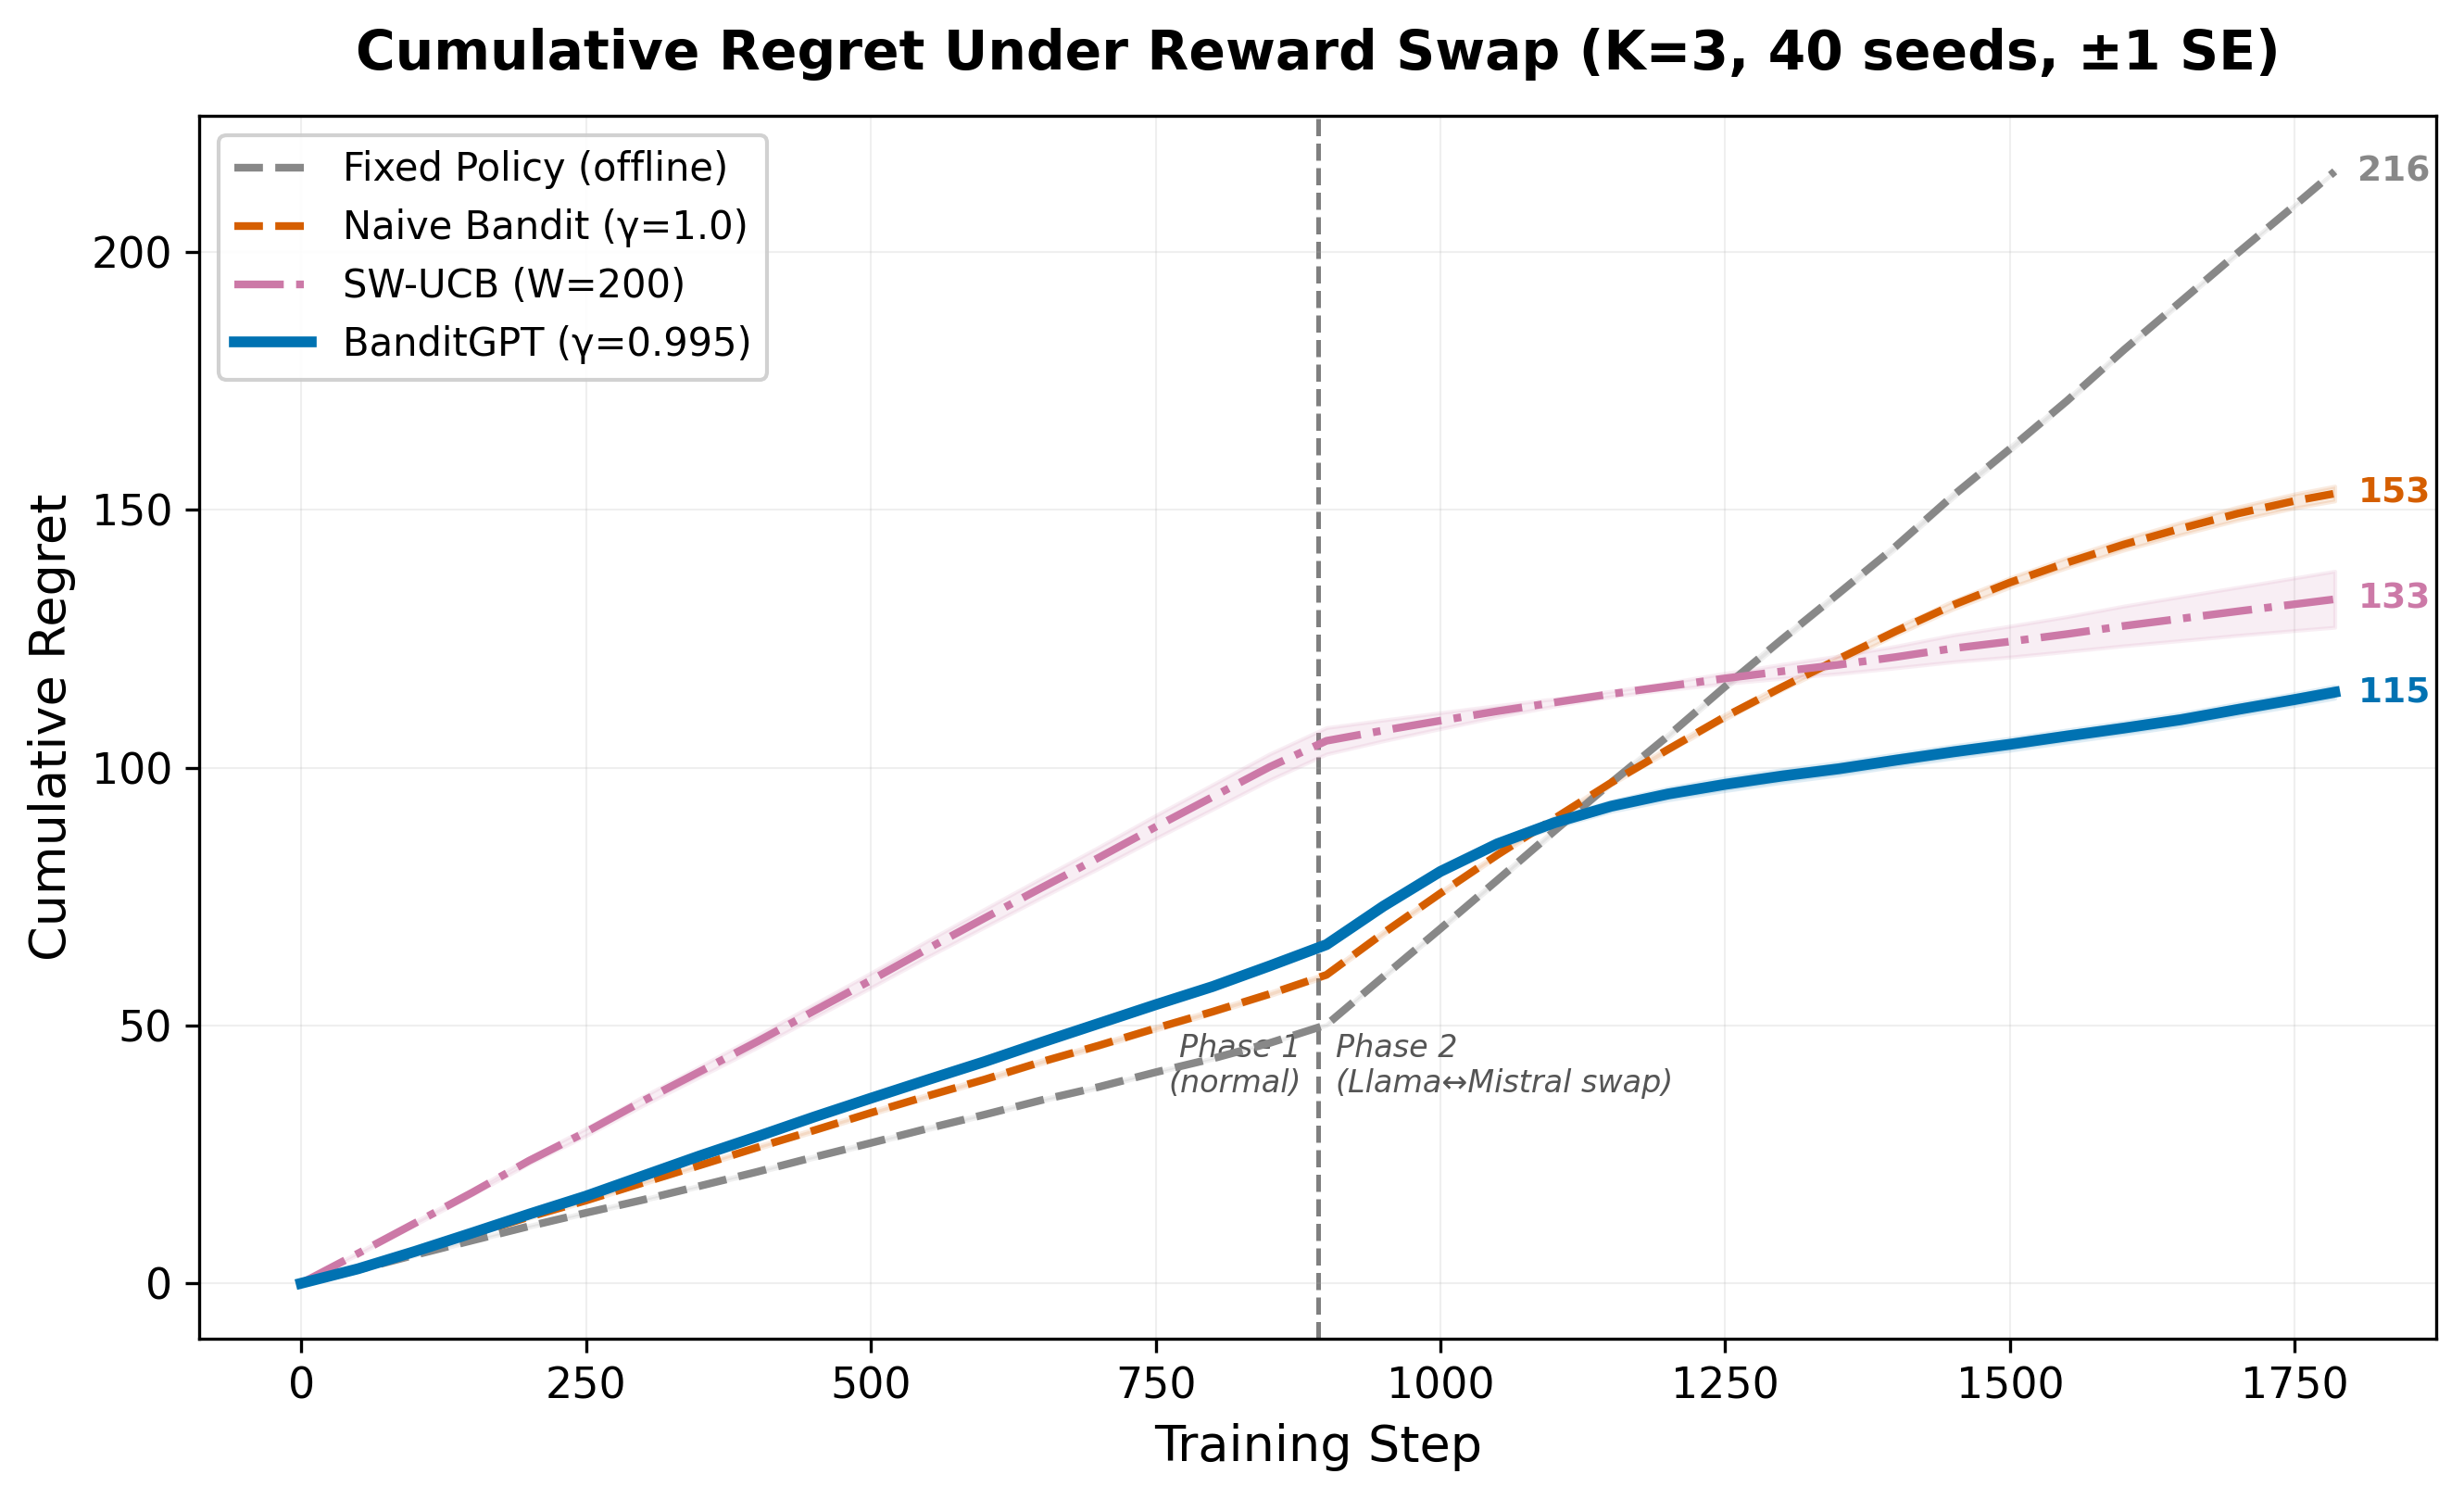
\includegraphics[width=\columnwidth]{figures/cumulative_regret.pdf}
\caption{Cumulative Regret under Reward Drift. BanditGPT ($\gamma=0.995$) adapts rapidly to quality degradation, unlike naive bandits or frozen policies.}
\label{fig:cumulative_regret}
\end{figure}

Beyond lower mean regret, BanditGPT exhibits the lowest cross-seed variance ($\sigma{=}7.2$), while the Naive Bandit's is $2.4\times$ higher ($\sigma{=}17.6$). Infinite memory creates sensitivity to the random ordering of observations, whereas geometric forgetting regularizes this variance, ensuring every deployment adapts reliably.

\subsection{Budget Pacing under Cost Drift}
\label{sec:exp3_cost_drift}

We now introduce the most complex and realistic scenario: a mid-stream price drop (Cost Drift) while operating under strict budget constraints. In Phase 2, Gemini-Pro's price drops to nearly zero. We evaluate three budget regimes: Tight (\$0.00023/req), Moderate (\$0.00066/req), and Loose (\$0.0019/req).

\paragraph{Budget compliance is the key differentiator.}
The Fixed Policy (using an offline-tuned static penalty $\lambda_s$) massively under-spends the target across all three budgets ($0.12\times$ to $0.49\times$). Because it cannot refine its reward estimates, its aggressive penalty prevents it from utilizing its full budget to maximize quality. The Naive Bandit is inconsistent: it tracks the target at tight and moderate budgets by coincidence, but over-spends by a massive $2.78\times$ at the loose budget because the static penalty cannot adjust. 

BanditGPT is the only system that reliably hits the budget in Phase 1 ($0.97\times$ to $1.00\times$ across all three targets; Table~\ref{tab:main_results}b). The BudgetPacer's primal-dual mechanism adjusts $\lambda_t$ continuously based on observed costs, providing closed-loop control that static penalties cannot replicate.

\paragraph{Exploiting the price drop.}
When Gemini becomes nearly free in Phase~2, the BudgetPacer automatically detects the cost reduction via its EMA signal.
The three budget regimes produce qualitatively distinct---but equally principled---dual-variable responses (Figure~\ref{fig:adaptation_dynamics}).
At moderate and loose targets, post-drop costs fall well below the budget ($0.51\times$ and $0.19\times$ respectively), so $\lambda_t$ decays to near-zero: the constraint becomes slack and the router reverts to quality-only optimization, increasing Gemini selection to ${\sim}47$--$49\%$.
At the tight target, the opposite occurs: post-drop costs (\$2.38e-4/req) slightly exceed the budget (\$2.34e-4), so $\lambda_t$ \emph{rises} from $0.46$ to $0.82$.
Paradoxically, this elevated dual variable produces the \emph{highest} Gemini adoption ($84\%$) of any constrained condition, because the soft penalty $\lambda_t \times \tilde{c}_m$ penalizes the now-expensive Mistral ($\tilde{c}{=}0.49$) far more than the now-cheap Gemini ($\tilde{c}{\approx}0$).
All three regimes show highly significant reward lifts ($\Delta{=}+0.017$ to $+0.065$; $p < 10^{-9}$), with the tight budget exhibiting the largest gain precisely because its binding constraint concentrates traffic on the cost-efficient frontier.

\begin{figure*}[t]
\centering

\includegraphics[width=\textwidth]{figures/adaptation_dynamics.pdf}
\caption{Adaptation dynamics under cost drift (50~seeds, $\pm$1\,SE shading).
At step~912, Gemini-2.5-Pro's price drops to near-zero.
At moderate/loose budgets, $\lambda_t$ decays to zero (slack constraint) and Gemini rises to ${\sim}47$--$49\%$.
At the tight budget, $\lambda_t$ \emph{rises} (binding constraint) and Gemini surges to $84\%$---the pacer concentrates traffic on the cheapest high-quality arm while maintaining $1.02\times$ budget compliance.}
\label{fig:adaptation_dynamics}
\end{figure*}

\paragraph{Tight budgets: binding constraints as a feature.}
A particularly instructive result emerges at the tight target ($B{=}\$0.00023$/req).
Rather than being a limitation, the tight budget produces the \emph{strongest} adaptation:
BanditGPT achieves $84\%$ Gemini selection in Phase~2 (vs.\ $47$--$49\%$ for moderate/loose) and the largest reward lift ($\Delta{=}+0.065$).
This occurs because the dual variable $\lambda_t$ rises to $0.82$ when costs slightly exceed the tight target, creating a large soft-penalty gap between the now-cheap Gemini and the now-expensive Mistral.
Meanwhile, the Fixed Policy and Naive Bandit---using static cost penalties---overshoot the tight budget by $11$--$13\%$ in Phase~2 because their open-loop penalties cannot adapt to the new cost landscape.
BanditGPT stays within $2\%$ of target, demonstrating that the primal-dual mechanism provides precise closed-loop budget control under non-stationary pricing.

\subsection{Hyperparameter Selection via Epsilon-Constraint}
\label{sec:exp4_hparam_sweep}

Selecting hyperparameters ($\alpha$, $n_\mathit{eff}$, $\gamma$) for a non-stationary router poses a fundamental tension: standard cross-validation maximises stationary quality and selects $\gamma{=}1.0$ (no forgetting), yet Section~\ref{sec:exp2_reward_shift} showed that $\gamma{=}1.0$ fails to adapt under distribution drift.  We resolve this with the \textbf{epsilon-constraint method}, a principled bi-objective selection procedure.

\paragraph{Two objectives.}
Each configuration in the grid ($6 \times 6 \times 4$ values of $\alpha$, $n_\mathit{eff}$, $\gamma$) is scored on two metrics using the validation split:
\begin{enumerate}[nosep,leftmargin=*]
  \item \emph{Budget-paced Pareto AUC} (primary): the area under the quality--cost Pareto frontier when sweeping budget targets with the BudgetPacer active. Higher is better.
  \item \emph{Phase-2 cumulative regret} (secondary): a two-phase simulation where, at the midpoint, two arms swap their reward \emph{and} cost distributions. Only post-swap regret is recorded, averaged over all $\binom{K}{2}$ swap pairs and 10 seeds. Lower is better.
\end{enumerate}

\paragraph{Selection rule.}
Among all configurations whose budget-paced AUC is within $\epsilon{=}5\%$ of the best, we select the one with the lowest Phase-2 regret.  This gives budget-pacing explicit priority---no configuration is chosen that materially degrades stationary routing---while using adaptation speed as the tiebreaker within the near-optimal band.

\paragraph{Result.}
Figure~\ref{fig:epsilon_tradeoff} visualises the tradeoff.  Configurations with $\gamma{=}1.0$ (blue) achieve the highest AUC but the worst post-swap regret: they cannot shed stale evidence.  Lower $\gamma$ values shift points downward (better adaptation) at only marginal AUC cost---all 144 BanditGPT configurations fall within the $\epsilon$-feasible band, confirming that stationary routing quality is robust across the grid.  Because the entire grid is feasible, Phase-2 regret becomes the effective tiebreaker.  The method selects $\gamma{=}0.995$ (star), which reduces Phase-2 regret by 12\% compared to the AUC-only winner ($\gamma{=}1.0$, red~\textbf{X}: regret $79.2 \to 69.6$) while sacrificing only 0.25\% of stationary AUC.  This configuration defines a ${\sim}200$-step effective memory window---long enough for stable exploitation, short enough to track realistic cost and quality shifts.

\begin{figure}[h]
\centering
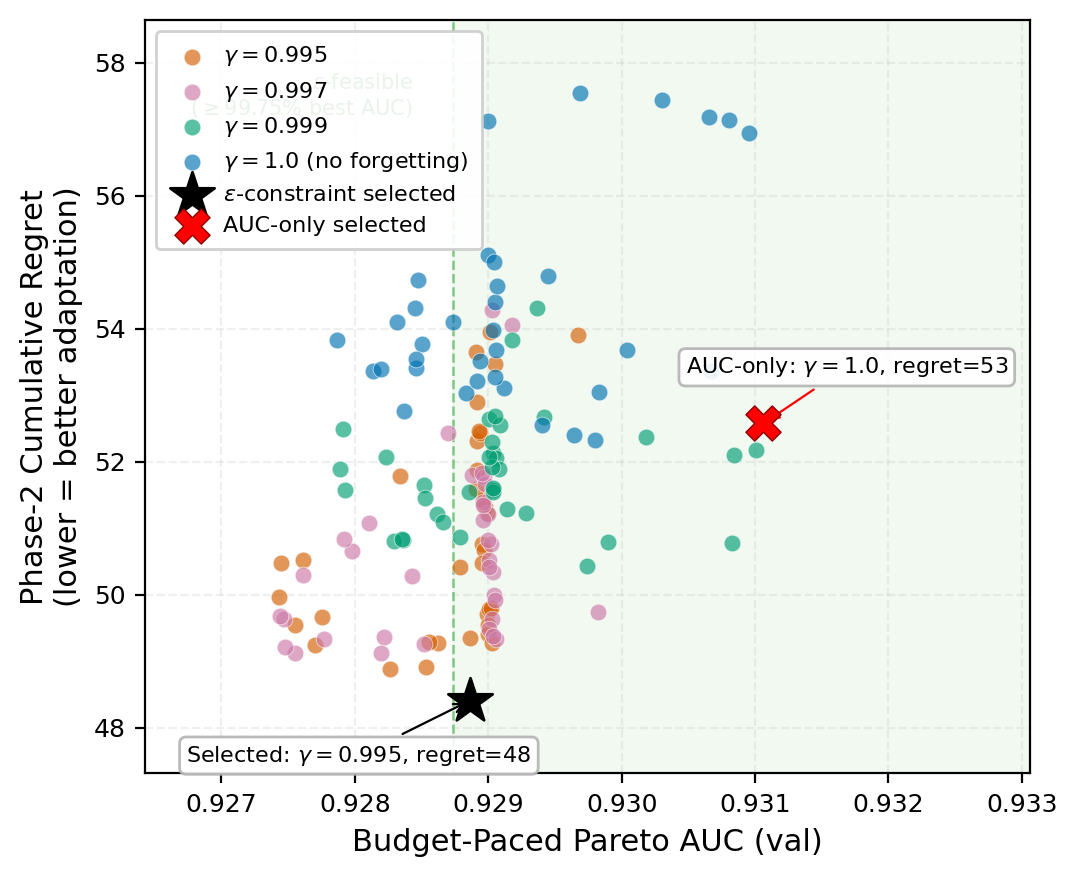
\includegraphics[width=\columnwidth]{figures/epsilon_tradeoff.pdf}
\caption{Efficiency--adaptability tradeoff for BanditGPT ($K{=}3$, PCA-25).  Each point is one ($\alpha$, $n_\mathit{eff}$, $\gamma$) configuration; colour encodes $\gamma$.  The green band marks the $\epsilon$-feasible region ($\geq$95\% of best AUC).  The black star is the $\epsilon$-constraint winner; the red \textbf{X} is the AUC-only winner ($\gamma{=}1.0$), which suffers the highest Phase-2 regret.}
\label{fig:epsilon_tradeoff}
\end{figure}